\documentclass[journal=asbcd6,manuscript=article]{achemso}

\usepackage{natbib}
\usepackage{setspace}
\usepackage{xkeyval}
\usepackage{array}
\usepackage{listings}
\usepackage{lmodern}
\usepackage{mathpazo}
\usepackage{geometry}
\usepackage{microtype}
\usepackage{url}  % Formatting web addresses
\usepackage{ifthen}  % Conditional
\usepackage{multicol}   %Columns
\usepackage[utf8]{inputenc} %unicode support
\usepackage{amsmath}
\usepackage{amssymb}
\usepackage{mathtools}
\usepackage{epsfig}
\usepackage{epstopdf}
\usepackage{graphicx}
\usepackage{textcomp}
\usepackage{multirow}
\usepackage{booktabs}
\usepackage{natmove}
\usepackage{float}
\usepackage[margin=0.1pt,font=footnotesize,labelfont=bf]{caption}
\usepackage[version=3]{mhchem} % Formula subscripts using \ce{}
\usepackage[T1]{fontenc}       % Use modern font encodings
%\usepackage[square,sort,comma,numbers,sort&compress]{natbib}
%%%%%%%%%%%%%%%%%%%%%%%%%%%%%%%%%%%%%%%%%%%%%%%%%%%%%%%%%%%%%%%%%%%%%
%% If issues arise when submitting your manuscript, you may want to
%% un-comment the next line.  This provides information on the
%% version of every file you have used.
%%%%%%%%%%%%%%%%%%%%%%%%%%%%%%%%%%%%%%%%%%%%%%%%%%%%%%%%%%%%%%%%%%%%%
%%\listfiles

%\bibliographystyle{achemso}
\newcommand*\mycommand[1]{\texttt{\emph{#1}}}
%%%%%%%%%%%%%%%%%%%%%%%%%%%%%%%%%%%%%%%%%%%%%%%%%%%%%%%%%%%%%%%%%%%%%

%%%%%%%%%%%%%%%%%%%%%%%%%%%%%%%%%%%%%%%%%%%%%%%%%%%%%%%%%%%%%%%%%%%%%
\author{Michael Vilkhovoy}
\affiliation[Cornell University]
{Robert Frederick Smith School of Chemical and Biomolecular Engineering, Cornell University, Ithaca, NY 14853}
\author{Nicholas Horvath}
\affiliation[Cornell University]
{Robert Frederick Smith School of Chemical and Biomolecular Engineering, Cornell University, Ithaca, NY 14853}
\author{Joseph Wayman}
\affiliation[Cornell University]
{Robert Frederick Smith School of Chemical and Biomolecular Engineering, Cornell University, Ithaca, NY 14853}
\author{Kara Calhoun}
\affiliation[Stanford University]
{School of Chemical Engineering, Stanford University, Stanford, CA 94305}
\author{James Swartz}
\affiliation[Stanford University]
{School of Chemical Engineering, Stanford University, Stanford, CA 94305}
\author{Jeffrey D. Varner}
\email{jdv27@cornell.edu}
\phone{+1~(607)~255-4258}
\fax{+1~(607)~255-9166}
\affiliation[Cornell University]
{Robert Frederick Smith School of Chemical and Biomolecular Engineering, Cornell University, Ithaca, NY 14853}
%%%%%%%%%%%%%%%%%%%%%%%%%%%%%%%%%%%%%%%%%%%%%%%%%%%%%%%%%%%%%%%%%%%%%
\title{Sequence Specific Modeling of Cell-Free Protein Synthesis}
%\abbreviations{MV,NH,JDV}
\keywords{Synthetic biology, constraints based modeling, cell-free protein synthesis}

\begin{document}

%%%%%%%%%%%%%%%%%%%%%%%%%%%%%%%%%%%%%%%%%%%%%%%%%%%%%%%%%%%%%%%%%%%%%
%% The abstract environment will automatically gobble the contents
%% if an abstract is not used by the target journal.
%%%%%%%%%%%%%%%%%%%%%%%%%%%%%%%%%%%%%%%%%%%%%%%%%%%%%%%%%%%%%%%%%%%%%
\begin{abstract}
In this study, we used sequence specific constraints based modeling to evaluate the performance of synthetic circuits in an \emph{E.~coli} cell-free protein synthesis system.
A core \emph{E.~coli} metabolic model, consisting of glycolysis, pentose phosphate pathway, amino acid biosynthesis and degradation and energy metabolism, was then augmented with sequence specific descriptions of genetic circuits which included mechanistic models of promoter function, transcription and translation.
Thus, unlike other synthetic biology modeling efforts, sequence specific constraints based modeling explicitly couples the transcription and translation of circuit components with the availability of metabolic resources.
Model parameters for transcription and translation were taken from literature, allowing a first principles prediction of circuit performance.
We tested this approach by first simulating T7 induced chloramphenicol acetyltransferase production and $\sigma_{70}$-induced deGFP expression; we then expanded these studies for a range of different proteins.
First principles predictions of circuit performance were consistent with measurements for a variety of cases.
Further, global sensitivity analysis identified the key metabolic processes that controlled circuit performance in terms of productivity, energy efficiency, and carbon yield.
A sufficient energy supply with oxidative phosphorylation is instrumental for high energy efficiency and carbon yields; in addition, the translation rate could be optimized for higher productivity.
Taken together, sequence specific constraints based modeling offers a novel means to \emph{a~priori} estimate the performance of cell-free synthetic circuits.
\end{abstract}

%%%%%%%%%%%%%%%%%%%%%%%%%%%%%%%%%%%%%%%%%%%%%%%%%%%%%%%%%%%%%%%%%%%%%
%% Start the main part of the manuscript here.
%%%%%%%%%%%%%%%%%%%%%%%%%%%%%%%%%%%%%%%%%%%%%%%%%%%%%%%%%%%%%%%%%%%%%

\section{Introduction}
Cell-free systems offer many advantages for the study, manipulation and modeling of metabolism compared to \textit{in~vivo} processes.
Central amongst these advantages is direct access to metabolites and the microbial biosynthetic machinery without the interference of a cell wall.
This allows us to control as well as interrogate the chemical environment while the biosynthetic machinery is operating, potentially at a fine time resolution.
Second, cell-free systems also allow us to study biological processes without the complications associated with cell growth.
Cell-free protein synthesis (CFPS) systems are arguably the most prominent examples of cell-free systems used today \cite{Jewett:2008aa}.
However, CFPS is not new; CFPS in crude \textit{E.~coli} extracts has been used since the 1960s to explore fundamentally important biological mechanisms \cite{MATTHAEI:1961aa,NIRENBERG:1961aa}.
Today, cell-free systems are used in a variety of applications ranging from therapeutic protein production \cite{Lu:2014aa} to synthetic biology \cite{Hodgman:2012aa}.
Interestingly, many of the challenges confronting \textit{in~vivo} genome scale kinetic modeling can potentially be overcome in a cell-free system.
For example, there is no complex transcriptional regulation to consider, transient metabolic measurements are easier to obtain, and we no longer have to consider cell growth.
Thus, cell-free operation holds several significant advantages for model development, identification and validation.
Theoretically, genome scale cell-free kinetic models may be possible for industrially important organisms, such as \textit{E.~coli} or \textit{B. subtilis}, if a simple, tractable framework for integrating allosteric regulation with enzyme kinetics can be formulated.

Stoichiometric reconstructions of microbial metabolism popularized by constraints based modeling techniques such as flux balance analysis (FBA) have become standard tools to interrogate biological networks \cite{2012_lewis_palsson_NatRevMicrobio}.
Since the first genome scale stoichiometric model of \textit{E.~coli}, developed by Edwards and Palsson \cite{2000_edwards_palsson_PNAS}, stoichiometric reconstructions of hundreds of organisms including industrially important prokaryotes such as \textit{E.~coli} \cite{Feist:2007aa} or \textit{B. subtilis} \cite{Oh:2007aa} are now available \cite{2009_feist_palsson_NatRevMicrobio}.
Traditionally, stoichiometric models have also neglected explicit descriptions of metabolic regulation and control mechanisms, instead opting to describe the choice of pathways by prescribing an objective function on metabolism.
Interestingly, similar to early cybernetic models, the most common metabolic objective function has been the optimization of biomass formation \cite{2002_ibarra_edwards_palsson_Nat}, although other metabolic objectives have also been estimated \cite{2007_schuetz_sauer_MolSysBio}.
Recent advances in constraints based modeling have overcome the early shortcomings of the platform, including capturing metabolic regulation and control \cite{2013_hyduke_lewis_palsson_MolBioSys}. Thus, modern constraints based approaches are extremely useful for the discovery of metabolic engineering strategies and represent the state of the art in metabolic modeling \cite{2013_mccloskey_palsson_feist_MolSysBio, 2012_zomorrodi_maranas_MetaEng}.

In this study, we used sequence specific constraints based modeling to evaluate the performance of synthetic circuits in an \emph{E.~coli} cell-free protein synthesis (CFPS) system.
A core \emph{E.~coli} cell-free metabolic model, consisting of 132 metabolites and 281 reactions, was developed from literature \cite{Feist:2007aa}.
This model, which described glycolysis, pentose phosphate pathway, amino acid biosynthesis and degradation and energy metabolism, was then augmented with
sequence specific descriptions of genetic circuits which included mechanistic models of promoter function, transcription and translation.
Thus, sequence specific constraints based modeling explicitly coupled the transcription and translation of circuit components with the availability of metabolic resources.
We tested this approach by first simulating the production of CAT and deGFP under two different promoters, and then expanded this for $\sigma_{70}$-induced deGFP expression at different plasmid concentrations.
First principles predictions of circuit performance were consistent with measurements.
We then investigated the productivity and carbon yield for a range of 8 different proteins for a variety of cases.
From this, higher carbon number proteins typically had lower productivity rates and carbon yields than that of the lower carbon number proteins.
Further, global sensitivity analysis identified the key metabolic processes that controlled circuit performance, showing oxidative phosphorylation as instrumental for maintaining a high carbon yield and the translation rate for productivity.
Taken together, sequence specific constraints based modeling offers a novel means to \emph{a~priori} estimate the performance of cell-free synthetic circuits.

\section{Results and discussion}

\subsection{Model Derivation}
The goal of this work was first to construct a modeling framework to describe cell-free protein synthesis systems and to examine its performance in productivity, energy efficiency and carbon yield for a protein of interest.
One mathematical framework that has found wide use in modeling metabolism is constraints based models such as flux balance analysis (FBA).
FBA can predict how cells utilize nutrients to produce products by using the biochemical stoichiometry and thermodynamical feasibility under pseudo steady-state conditions.
Traditionally, FBA is used to model \textit{in~vivo} processes; however, cell-free systems do not have growth associated reactions or transport through the cell membrane.
Thus, to model cell-free metabolism we constructed a stoichiometric network by removing growth associated reactions from the \textit{i}AF1260 reconstruction of K-12 MG1655 \textit{E.~coli} \cite{Feist:2007aa}, and incorporating amino acid synthesis and transcription/translation associated reactions \cite{Allen:2003aa} for a protein of interest to be expressed.
The network consisted of 272 reactions and 145 species.
The core metabolism is shown in Fig.~\ref{fig:network}A.
We developed a cell-free sequence specific flux balance analysis (ssFBA) with a detailed promoter model \cite{Moon:2012aa} to examine the performance of CFPS.
We first validated the ssFBA approach by comparing simulated and measured concentrations of two proteins from two different cell-free \textit{E.~coli} extract systems.
The first protein, chloramphenicol acetyltransferase (CAT), was produced under a T7 promoter in a glucose/NMP cell-free system \cite{2005_calhoun_BiotechnologyProgress} for a duration of 1 hour under glucose consumption (Fig.~\ref{fig:network}B).
The second protein, dual emission green fluorescent protein (deGFP), was produced under a P70 promoter in TXTL 2.0 \textit{E.~coli} extract for a duration of 8 hours under maltose consumption (Fig.~\ref{fig:network}C).
The ssFBA simulations predicted the production of both proteins for the duration of both CFPS batch reactions.
Uncertainty in experimental factors such as RNA polymerase, ribosome concentrations, elongation rates and the upper bounds for oxygen and glucose consumption rates did not alter the qualitative performance of the model.
Thus, the metabolic network and molecular description of trancription and translation were consistent with experimental measurements.
Next, ssFBA predicted deGFP production as a function of plasmid concentration (Fig.~\ref{fig:network}D).
Concentration of deGFP at each plasmid concentration was calculated by multiplying the flux of deGFP synthesis by the active time of production, approximately 8 hours in TXTL 2.0 \cite{Garamella:2016aa}.
The mean of the ensemble shows a good prediction against the measured deGFP levels, even though it under predicted deGFP concentration at the saturating point of 5 nM of plasmid concentration.
However, the ensemble and the mean of the ensemble captured the overall saturating dynamics of deGFP production as a function of plasmid concentration.
\begin{figure}[t!]
\centering
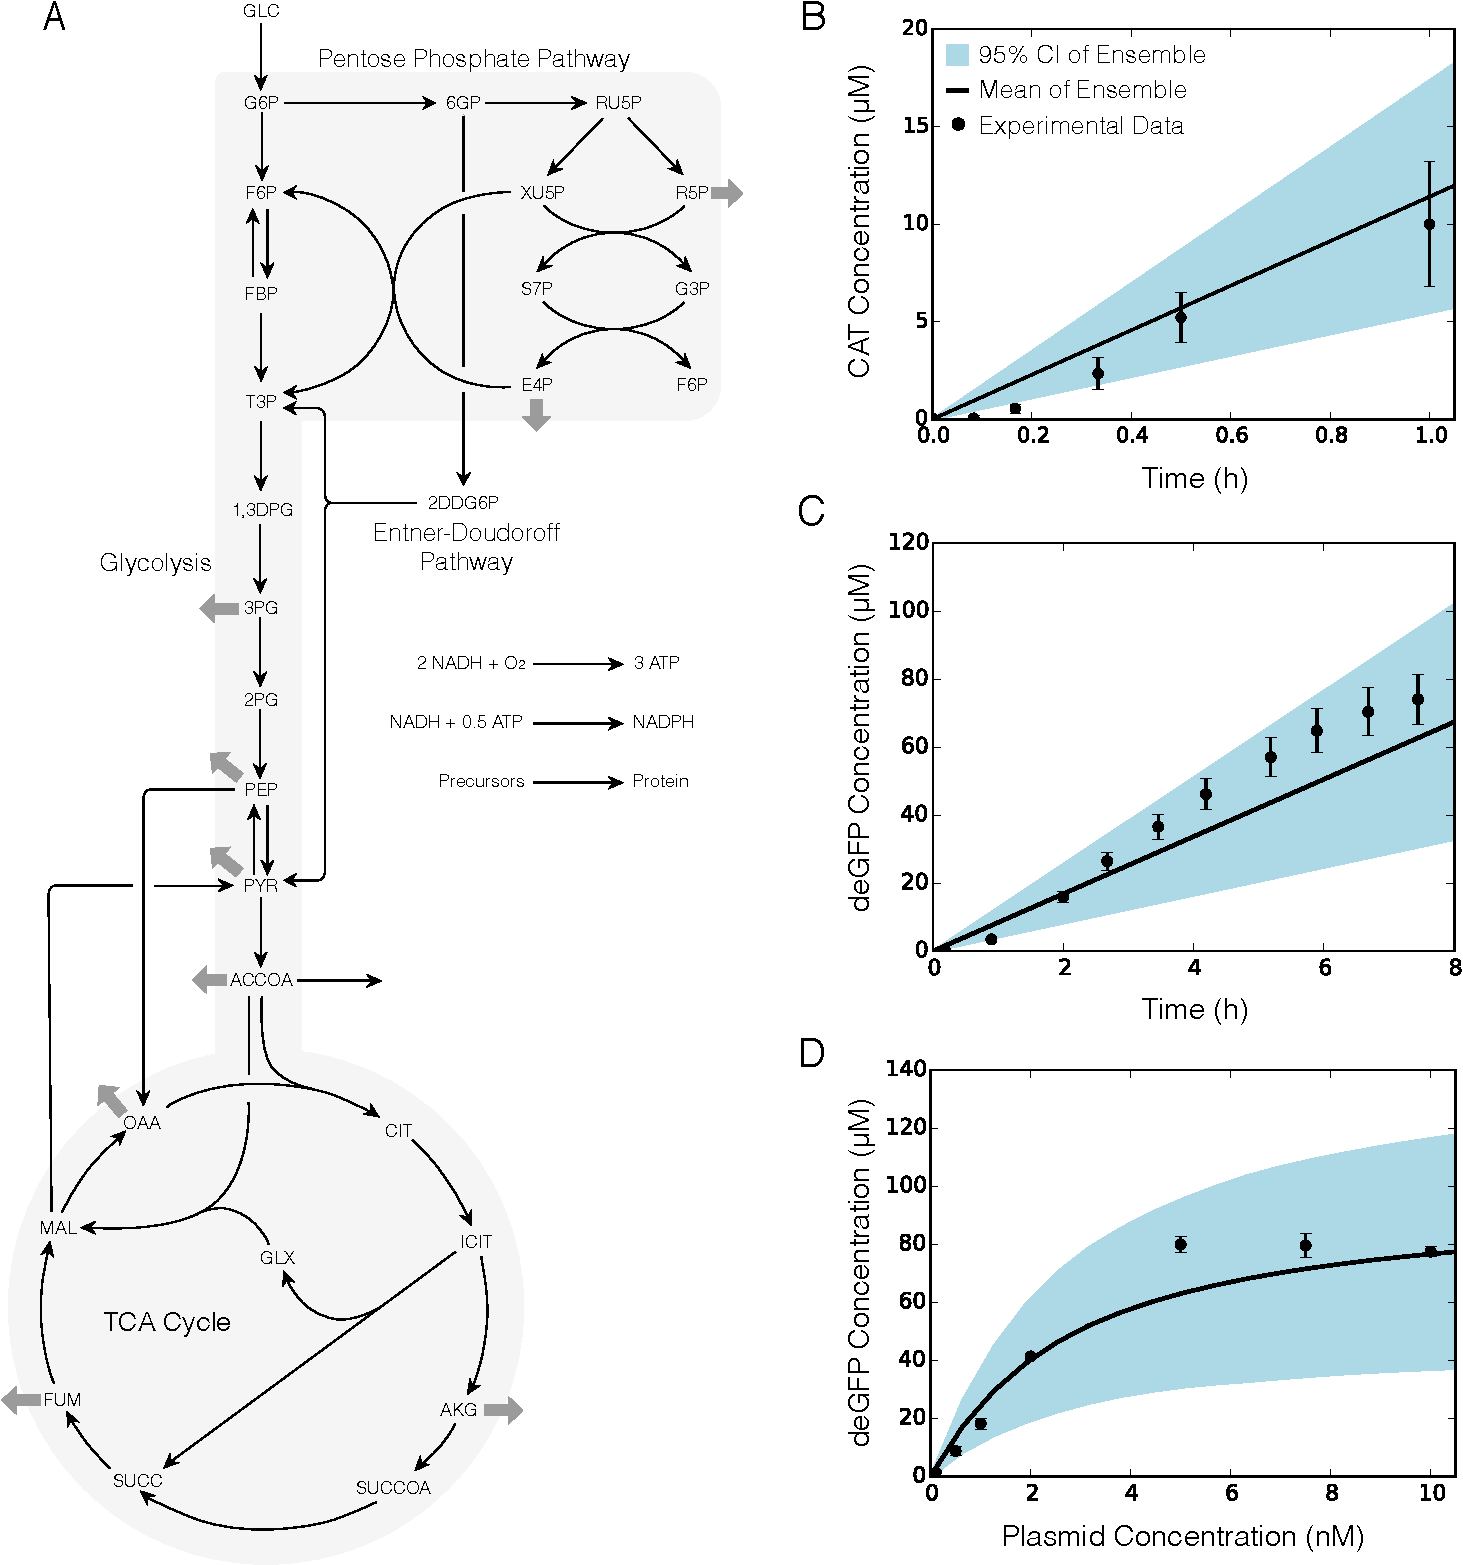
\includegraphics[width=1.00\textwidth]{./Figures/ssFBA_network.pdf}
\caption{Sequence specific flux balance analysis. A. Core metabolic network with glycolysis, pentose phoshate pathway, TCA cycle, Entner-Doudoroff pathway. Thick gray arrows indicate withdrawal of precursors for amino acid synthesis. B. CAT production under a T7 promoter in CFPS \textit{E.~coli} extract for 1 h under glucose consumption. C. deGFP production under a P70 promoter in TXTL 2.0 \textit{E.~coli} extract for 8 h under maltose consumption. D. Predicted deGFP concentration at different plasmid concentrations versus measurements of deGFP synthesized in TXTL 2.0. 95\% CI (blue region) over the ensemble of 100 sets, mean of the ensemble (black line), and experimental measurements (dots).}
\label{fig:network}
\end{figure}

These results validated our mathematical framework to model CFPS systems and predict the production of two proteins with few adjustable parameters in the promoter model taken from literature \cite{Moon:2012aa}.
It also showed that the sequence specific reactions were sufficient to predict the production of two different proteins under two different promoters and cell-free systems.
Since the model accurately predicted the behavior of protein production, we extended our mathematical framework to understand the performance limits of CFPS and how they could be addressed.

Our next goal was to examine the performance of CFPS for eight different proteins under three different cases.
Each of the proteins was produced under a P70 promoter, except for CAT which was produced under a T7 promoter.
In all cases, CFPS was supplied with glucose.
In the first case, CFPS was supplied with amino acids, and the system was allowed to synthesize amino acids (AA uptake and synthesis).
In the second case, CFPS was supplied with amino acids, but the amino acid synthesis reactions were turned off (AA uptake w/o synthesis).
These amino acid synthesis reactions were blocked since during the cell-free extract preparation the cells are often supplied with amino acids; thus, the enzymes responsible for amino acid synthesis would not be present.
In the third case, CFPS was not supplied with amino acids, but the system could synthesize them (AA synthesis w/o uptake).  
Eight different proteins, ranging in size, were selected to evaluate CFPS performance: bone morphogenetic protein 10 (BMP10), chloramphenicol acetyltransferase (CAT), caspase 9 (CASP9), dual emission green fluorescent protein (deGFP), prothrombin (FII), coagulation factor X (FX), fibroblast growth factor 21 (FGF21), and single chain variable fragment R4 (scFvR4).
We used ssFBA to estimate the productivity for each of these proteins for each case (Fig.~\ref{fig:Prod}).
An additional case was considered for CAT, since a comprehensive dataset is available \cite{2005_calhoun_BiotechnologyProgress}; in this case, fluxes were constrained to experimental measurements where avaliable, with the exception of CAT production which was determined by the transcription/translation parameters.

\subsection{CFPS Productivity}
We evaluated CFPS productivity for all eight proteins and for each case.
All cases had very similar performance for each protein and were within a standard deviation of each other (Fig.~\ref{fig:Prod}A).
%with the second case (without amino acid synthesis) having a slightly higher productivity for most proteins.
The model framework is setup to optimize for the production of each protein and is constrained by the translation rate.  
This shows the system had sufficient substrates and metabolic precursors to power CFPS and synthesize each protein of interest with the same productivity, regardless of the case.
However, each protein had a different level of productivity.
For instance, BMP10 had a productivity of about 2.5 $\mu$M/h whereas CAT had a productivity of about 12 $\mu$M/h.
To examine this further, the mean productivity was plotted against the carbon number of each protein (Fig.~\ref{fig:Prod}B).
The proteins with the highest productivity had the lowest carbon number, whereas proteins with low productivity had higher carbon numbers.
This inverse trend was due to the fact that larger proteins require more amino acids and substrates to assemble them, resulting in lower productivity given the same resources.
A single trendline for all cases shows the expected productivity in CFPS depending on the carbon number of the protein of interest (available in the Supporting Information).
CAT was an outlier for the trendline, even though it was in the same order of magnitude as the trendline.
The difference in the T7 and  $\sigma_{70}$ promoters did not alter the qualitative productivity performance of CAT.
The higher productivity of CAT compared to all other proteins was most likely due to the lower transcription requirement of cytidine triphosphate which allowed a higher flux for translation.
% a further study on the nucleotide and amino acid requirements of each protein and its effect on CFPS performance should be investigated.
\begin{figure}[t!]
\centering
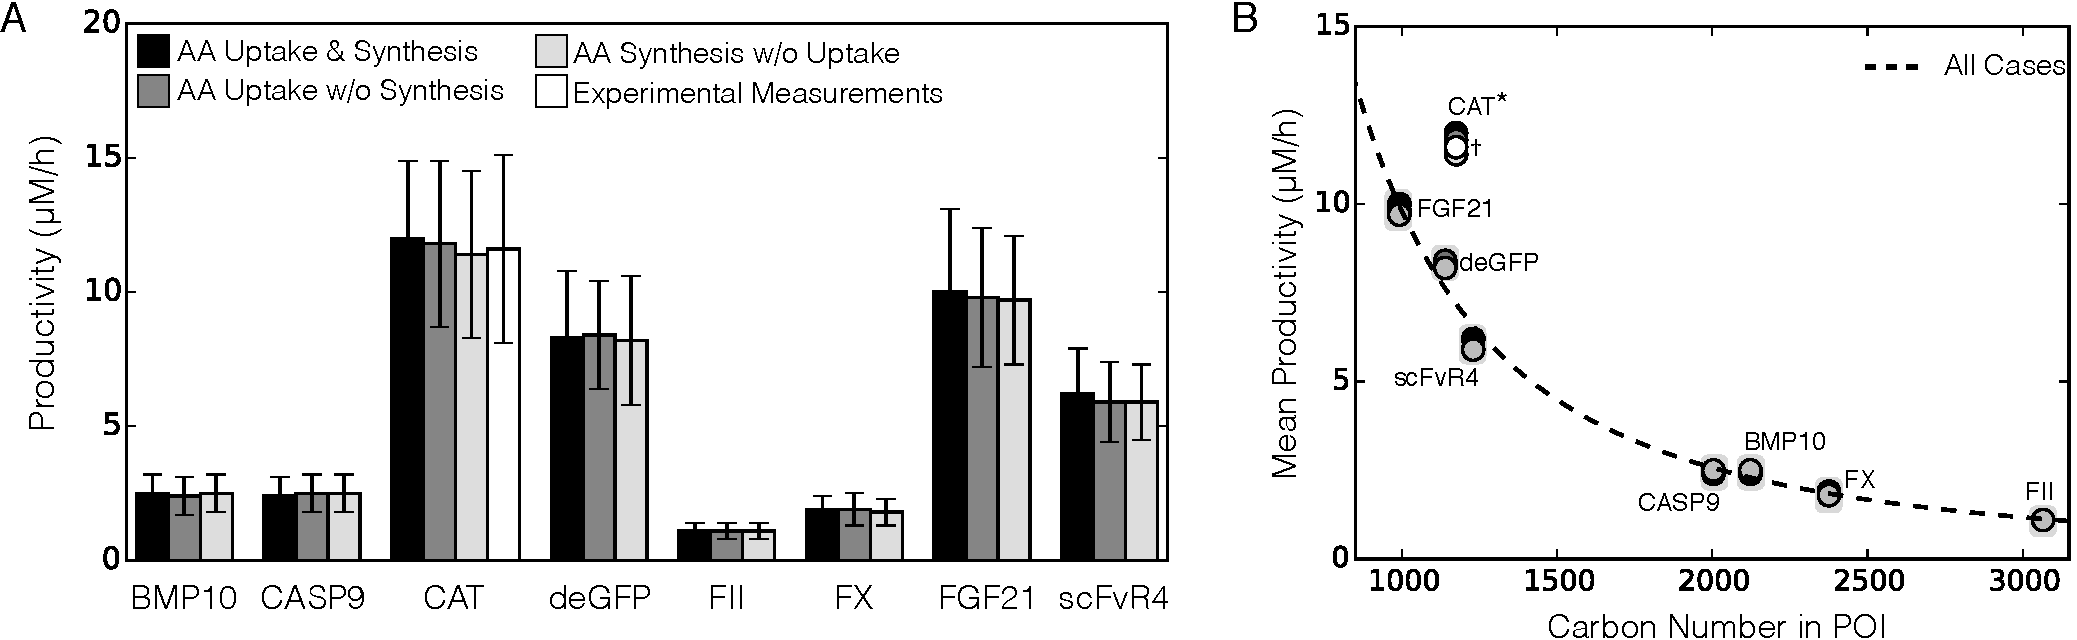
\includegraphics[width=1.00\textwidth]{./Figures/Productivity.pdf}
\caption{CFPS productivity of eight proteins for four cases. Amino acid uptake and synthesis (black), AA uptake without synthesis (dark grey), AA synthesis without uptake (light grey), and constrained by experimental measurements, for CAT only (white). A. Productivity across the ensemble (error bars represent 95\% CI). B. Mean productivity versus carbon number. Single trendline (dotted line) calculated across all cases (R\textsuperscript{2} = 0.99). Asterisk: protein excluded from trendline; dagger: constrained by experimental measurements and excluded from trendline.}
\label{fig:Prod}
\end{figure}
The drop in productivity in the third case is due to the fact that glucose is the only substrate supplied and must be used to provide the necessary energy requirements for transcription and translation, as well as synthesize each amino acid required for the production of the protein of interest.  

\subsection{CFPS Energy Efficiency}
Following the same outline as in examining the productivity, we calculated the energy efficiency of production for each protein (Fig.~\ref{fig:Energy}A).
The first two cases, where amino acids were supplied in the media, had comparable performance including having the highest energy efficiencies.
The third case (with no amino acid uptake) had the lowest energy efficiency; this was because glucose had to be utilized to synthesize the amino acids necessary for protein synthesis, in addition to being available for energy generation.
We next investigated the effect of protein carbon number on energy efficiency (Fig.~\ref{fig:Energy}B).
The same inverse trend was observed as for productivity, except that it was linear.
The proteins with the lowest carbon number had the highest energy efficiency and the higher carbon number proteins had a lower energy efficiency for the first two cases.
Proteins with a high carbon number have a higher transcription and translation cost then smaller proteins, leading to a lower energy efficiency of protein synthesis.  
The first two cases had the same trendline whereas for the third case there was a significant drop in energy efficiency which required its own trendline (available in the Supporting Information).
Interestingly, in the third case each protein had a similar energy efficiency of about 25\% regardless of carbon number.
In this case, the energy burden of synthesizing each amino acid required for the assembly of the protein kept the energy efficiency saturated at a relatively low level.
However, the experimentally constrained case of CAT production showed even a lower energy efficiency of 3.9 $\pm$ 1.5\% compared to the theoretical maximum of 72 $\pm$ 7.1\%.
This shows CFPS systems have a lot of room for improvement: first, the experimental setup still produced certain amino acids; these reactions could be turned off.
Second, the system had a high accumulation of metabolic byproducts, specifically organic acids, which is a result of inefficient energy utilization.

%This may be a potential area for improvement in CFPS to optimize for energy utilization.
\begin{figure}[t!]
\centering
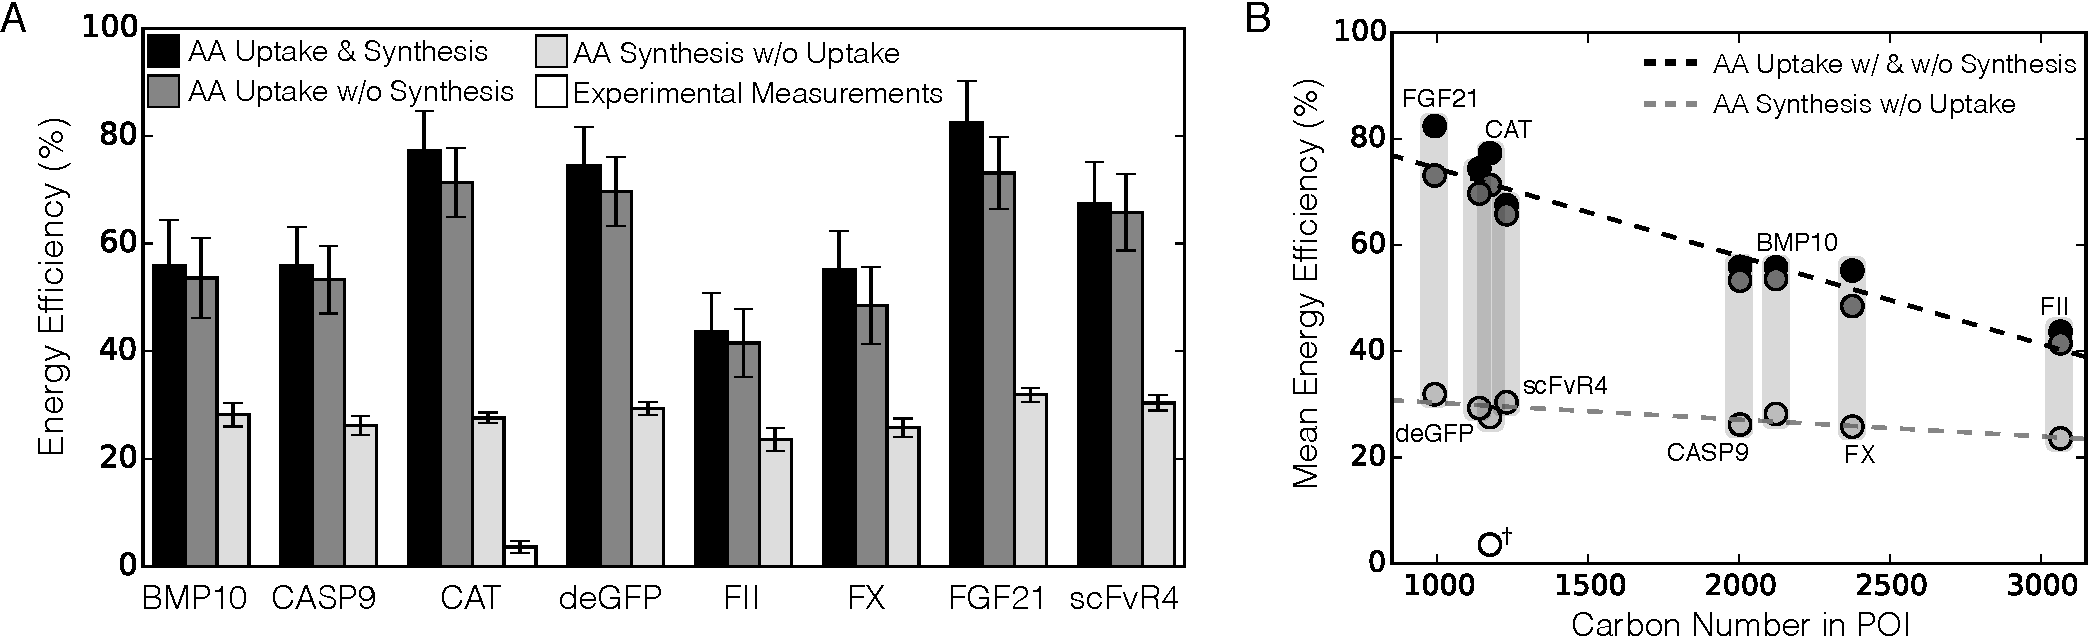
\includegraphics[width=1.00\textwidth]{./Figures/Energy.pdf}
\caption{CFPS energy efficiency of eight proteins for four cases. Amino acid uptake and synthesis (black), AA uptake without synthesis (dark grey), AA synthesis without uptake (light grey), and constrained by experimental measurements, for CAT only (white). A. Energy efficiency (Error bars represent the 95\% CI of the ensemble). B. Mean energy efficiency versus the carbon number for each corresponding protein. Trendline of energy efficiency versus carbon number (black dotted line) for first two cases  (R\textsuperscript{2} = 0.97) and trendline for AA synthesis without uptake (grey dotted line; R\textsuperscript{2} = 0.79). Dagger: constrained by experimental measurements and excluded from trendline.}
\label{fig:Energy}
\end{figure}


\subsection{CFPS Carbon Yield}
We also calculated the carbon yield for each protein (Fig.~\ref{fig:Yield}A).
The same trends followed, where the cases with amino acids supplied in the media showed the highest carbon yield.
The third case (with no amino acid uptake) had the lowest yields; this is most likely because glucose is utilized to synthesize the necessary amino acids for each protein as well as power the system.
%To determine the carbon contribution from each substrate (glucose and amino acids) we examined the carbon flux going toward the production of deGFP for all three cases (Table \ref{tbl:yield_breakdown}).
For the first case, the system relied on a mixture of glucose and some amino acids for each protein with a carbon yield of 56.9 $\pm$ 2.4\% for CAT.
Once amino acid synthesis was removed from the network (second case), each amino acid was utilized and the carbon yield increased to 57.0 $\pm$ 2.2\% for CAT.
Only the necessary amount of amino acids was used for the production of the protein of interest; thus, it may be hypothesized that all the glucose was used to power CFPS and did not contribute to the carbon yield.
In that case, the carbon yield without glucose contribution would be 100\%.
Finally, for the third case (without amino acids supplemented), the carbon yield was reduced to 51.1 $\pm$ 1.8\% for CAT, and the system used about twice the amount of glucose as in the first two cases.
In this case, glucose was used to synthesize amino acids and provide the energy necessary to power transcription and translation; this trend was seen across all proteins.
In the experimentally constrained case, CAT was produced with a carbon yield of 6\% compared to the theoretical maximum of 57\%.
This decrease in carbon yield suggests inefficiencies in CFPS that can potentially be improved.
ssFBA assumes a psuedo steady state; thus, intermediate metabolites cannot accumulate within the cell-free extract.
In addition, ssFBA is solved by setting protein production as the objective function.
Therefore, carbon flux will travel through the network to optimize the flux through the protein synthesis reaction.
In examining the experimental dataset, there is a high accumulation of organic acids, especially acetate.
The experimental performance could be improved by diverting this carbon toward the protein of interest by knockouts during the cell-free extract preparation.    
\begin{figure}[t!]
\centering
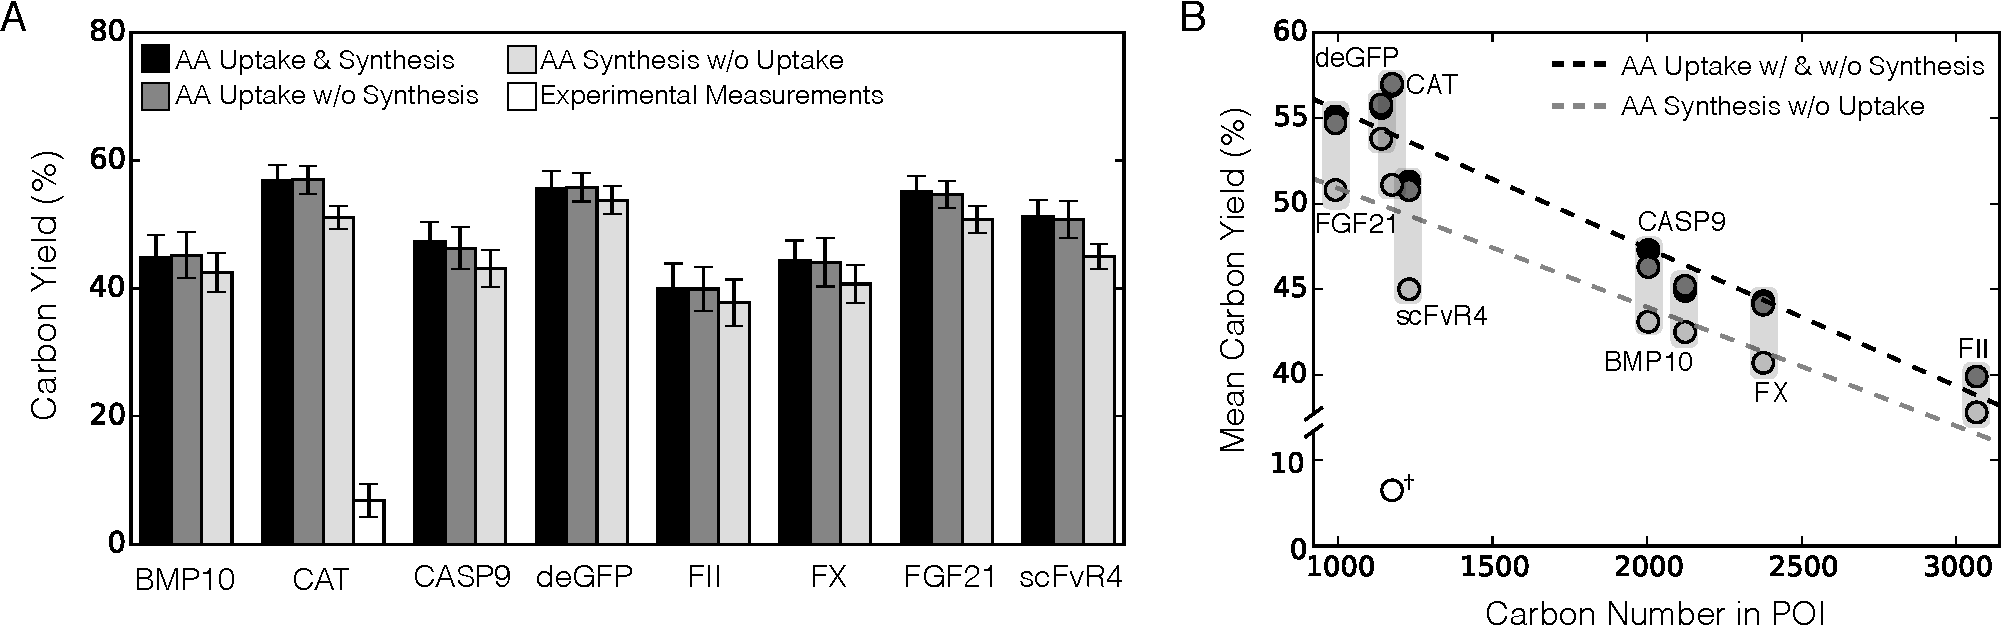
\includegraphics[width=1.00\textwidth]{./Figures/CarbonYield.pdf}
\caption{CFPS carbon yield of eight proteins for four cases. Amino acid uptake and synthesis (black), AA uptake without synthesis (dark grey), AA synthesis without uptake (light grey), and constrained by experimental measurements, for CAT only (white). A. Energy efficiency across the ensemble (error bars represent the 95\% CI). B. Mean energy efficiency versus the carbon number for each corresponding protein. Trendline of energy efficiency versus carbon number (black dotted line) for first two cases  (R\textsuperscript{2} = 0.92) and trendline for AA synthesis without uptake (grey dotted line; R\textsuperscript{2} = 0.83). Dagger: constrained by experimental measurements and excluded from trendline.}
\label{fig:Yield}
\end{figure}
Next we investigated the effect of the carbon number of each protein on the carbon yield (Fig.~\ref{fig:Yield}B).
The same inverse qualitative trend was observed as for productivity.
The proteins with the lowest carbon number had the highest yield and the higher carbon number proteins had a lower carbon yield within each case.
A single trendline was formulated for the first two cases since they had similar performance, while another trendline was formulated for the third cases (available in Supporting Information).
As the protein size increased, the carbon yield decreased, suggesting that large proteins may be less feasible for cell-free production.
Thus, we examined the parameters that had the most significant effect on cell-free productivity, energy efficiency, and carbon yield in order to optimize CFPS performance.

\subsection{CFPS performance sensitivity analysis}
To better understand the effect of substrate utilization and the transcription/translation parameters on CFPS performance we performed global sensitivity analysis on the productivity and energy efficiency for deGFP, a representative protein (Fig.~\ref{fig:SI}), as well as on the carbon yield (available in Supporting Information).
In examining productivity performance (Fig.~\ref{fig:SI}A), the significance of transcription/translation parameters was fairly constant across all three cases, with the rate of translation by ribosomes being the most significant.
As expected, this showed that the translation rate was instrumental for productivity, and should be the first step investigated during optimization, prior to examining transcription parameters.
Underwood and coworkers have also shown that an increase in ribosome levels did not significantly increase protein yields or rates; however, adding elongation factors increased yields by 23\% at 30 minutes \cite{2005_underwood_biotech}.
In addition, Li et al. have increased productivity of firefly luciferase by 5-fold in CFPS systems by adjusting factors that affect transcription and translation such as elongation factors, ribosome recycling factor, release factors, chaperones, BSA, and tRNAs \cite{2014_li_PlosOne}.
In examining substrate utilization, glucose uptake was not seen to be very important for productivity in the first two cases, but its significance increased when amino acids were removed from CFPS.
This makes sense, as amino acid synthesis from glucose became the only way to power protein synthesis in that case.
In addition, oxygen uptake had more significance in the third case than in the first two cases, since in that case oxygen was required to synthesize amino acids and power the system.
Also, oxygen determined how effectively glucose was utilized; therefore, if glucose uptake rate effects productivity, then oxygen could be expected to have a similar effect.
On the other hand, amino acid uptake showed significance for the first two cases, and was even higher for the second case (without AA synthesis), as it was the only source of amino acids.
\begin{figure}[t!]
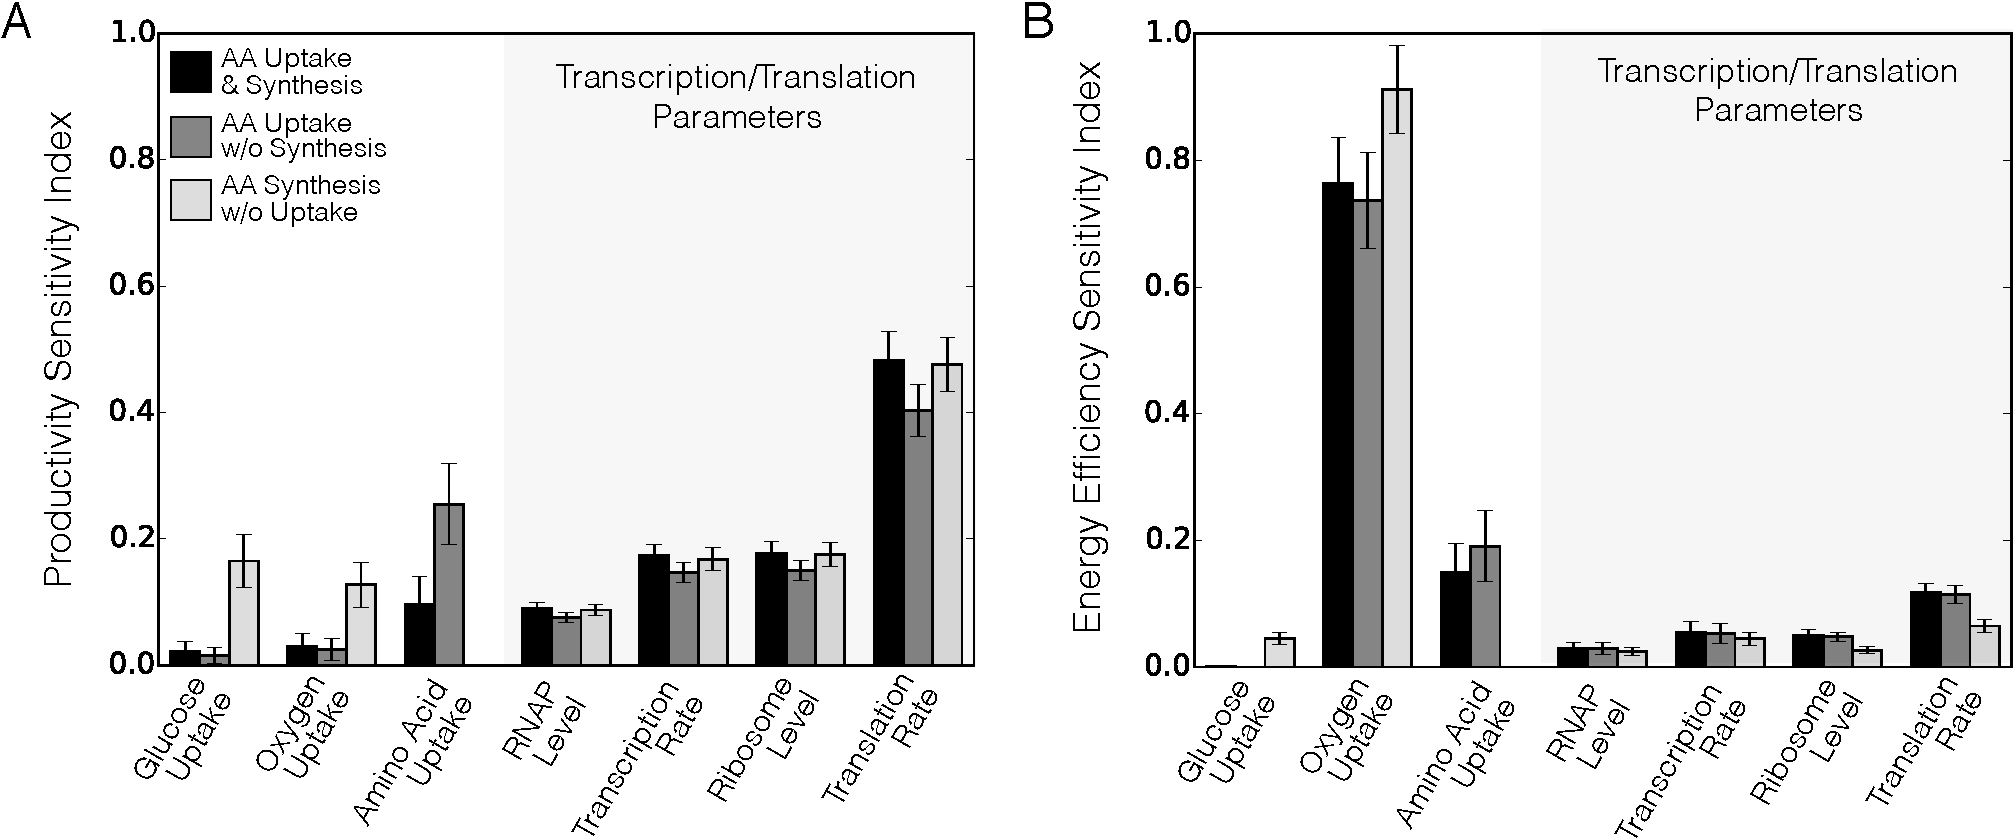
\includegraphics[width=1.00\textwidth]{./Figures/Sensitivity.pdf}
\caption{Total order sensitivity of deGFP productivity (A) and energy efficiency (B) to specific uptake rates and transcription/translation parameters for three cases: amino acid uptake and synthesis (black), amino acid uptake without synthesis (dark grey), and amino acid synthesis without uptake (light gray). Error bars represent a 95\% CI on the sensitivity index.}
\label{fig:SI}
\end{figure}

When considering energy efficiency performance (Fig.~\ref{fig:SI}B), the oxygen uptake rates were the most important for all three cases while the sensitivity to transcription/translation parameters decreased slightly.
The transcription/translation parameters had the same trend as for productivity, where the translation rate was the most sensitive compared to the other transcription/translation parameters and showed significance across all cases.
Thus, in investigating CFPS performance in terms of productivity and energy efficiency, the translation rate was an important parameter to optimize, as has already been shown in literature \cite{2005_underwood_biotech, 2014_li_PlosOne}.
Oxygen uptake showed significant importance for energy efficiency, since it was responsible for oxidative phosphorylation, the most efficieny pathway for energy generation.
Meanwhile, productivity was determined primarily by the rate of the most downstream steps, transcription and translation.
Across all three cases, substrate utilization (amino acid uptake and glucose) was shown to be the next most important as these substrates contributed to the carbon yield of deGFP.
In the first two cases where amino acids were supplied, amino acid uptake was significant, as without it energy was used to synthesize amino acids.
Glucose uptake was only seen to be significant in the third case, since it was the only source of carbon for protein synthesis and energy generation.
%This resulted in a tradeoff between energy generation to power transcription/translation and amino acid synthesis required to assemble the protein of interest.
Jewett and coworkers have reported that oxidative phosphorylation still operated in cell-free systems, and that yield decreased from 1.5-fold to 4-fold when oxidative phosphorylation reactions were knocked out in pyruvate-powered CFPS \cite{Jewett:2008aa}.
We also investigated the sensitivity of carbon yield to network fluxes; it followed the same trends as the energy efficiency sensitivity analysis.
It is unknown how active oxidative phosphorylation is compared to in \textit{in~vivo} systems.
To investigate this further we compared deGFP carbon yield to oxidative phosphorylation flux (Fig.~\ref{fig:oxphos_yield}).
Interestingly, oxidative phosphorylation has a strong effect on the carbon yield in all cases.
The first two cases follow the same trend, ranging from a carbon yield of 20\% to 55\%, depending on the oxidative phosphorylation activity.
The third case, followed the same trend; however, its carbon yield ranged from about 10\% to 55\%.  
The third case was expected to have a lower carbon yield for the same oxidative phosphorylation flux compared to the first two cases, since carbon must be utilized for energy generation and amino acid synthesis.
In all three cases, whenever the carbon yield was below its theoretical maximum, there was an accumulation of acetate and lactate, resulting in the lower carbon yield.
The experimental dataset exhibits a mixture of acetate and lactate accumulation during CAT synthesis, which shows that CFPS is not operating in a fully aerobic state.
It is unclear how active oxidative phosphorylation is in CFPS, since the reactions rely on electron transport from membrane vesicles.
The addition of phosphate showed an increase in CAT yield; however, it is unclear whether the addition of phosphate enhances oxidative phosphorylation, inhibits phosphatase reactions, or both \cite{Jewett:2008aa}.
Interestingly, the addition of NADH did not increase the rate of protein synthesis, since the concentration of ATP was most likely saturated.
An alternative strategy may be the inhibition of anaerobic processes in cell-free, in order to minimize unwanted byproducts such as acetate and lactate.
%Thus, it is interesting to see how much of the energetic needs of the system are met by oxidative phosphorylation and how much from anaerobic processes.
\begin{figure}[t!]
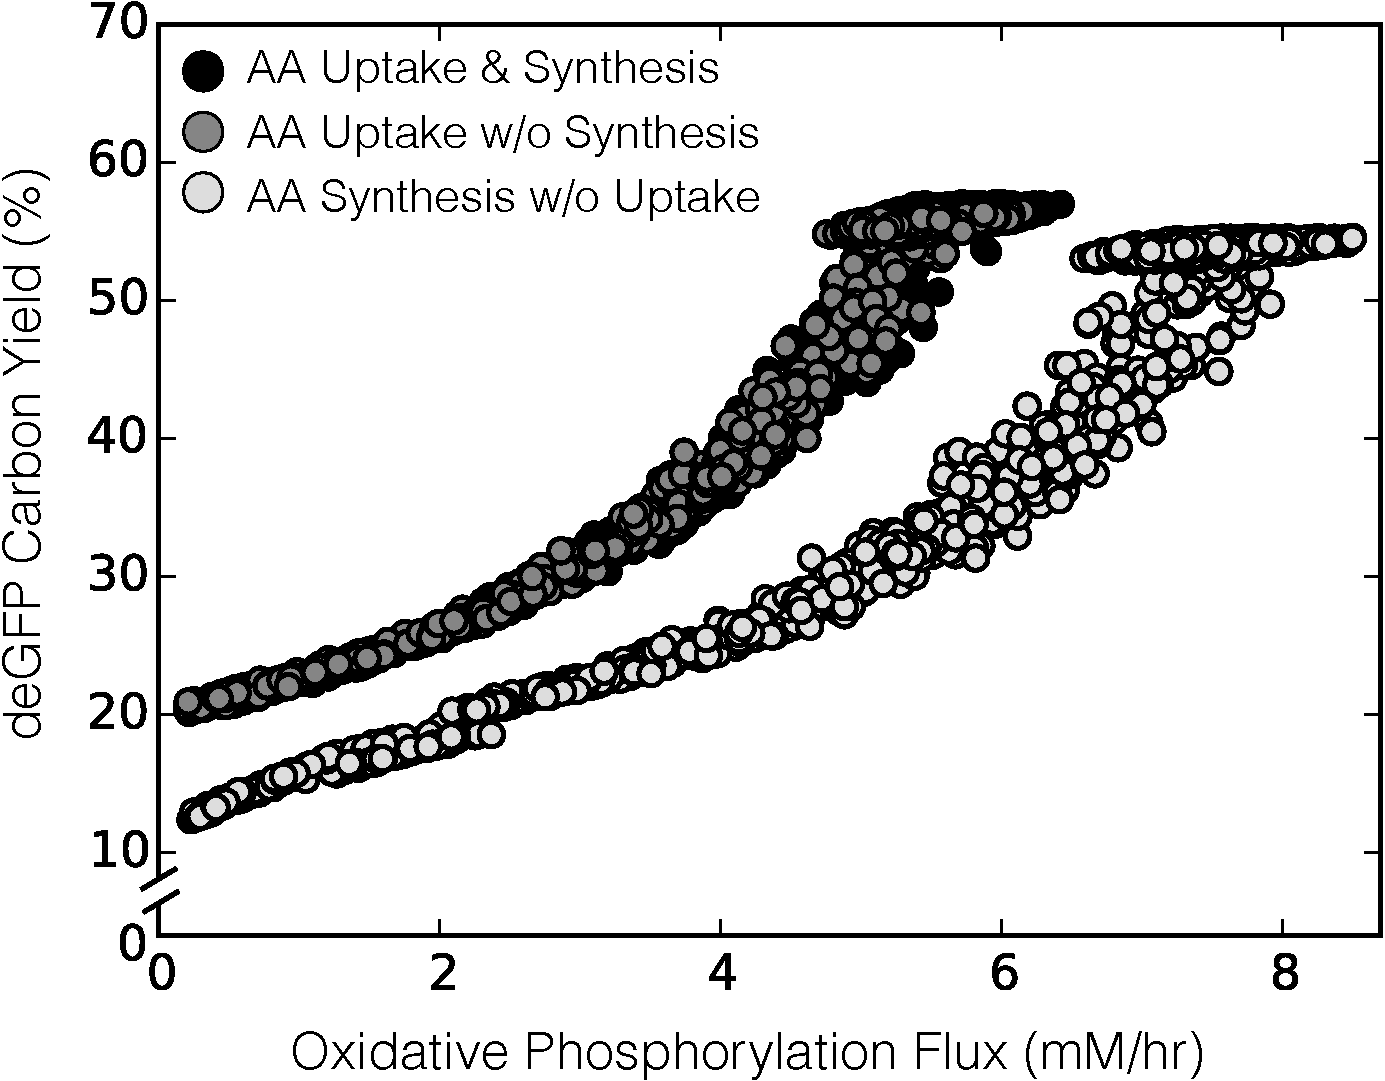
\includegraphics[width=0.7\textwidth]{./Figures/Yield_Ox.pdf}
\caption{deGFP carbon yield versus oxidative phosphorylation flux, across an ensemble of 1000 ssFBA solutions, for three cases: amino acid uptake and synthesis (black), amino acid uptake without synthesis (dark grey), and amino acid synthesis without uptake (light gray).}
\label{fig:oxphos_yield}
\end{figure}

To investigate the differences between the three cases, we compared the flux distributions for a representative protein, deGFP, predicted by ssFBA simulations, as well as the case constrained by experimental measurements for CAT (Fig.~\ref{fig:flux}).
\begin{figure}[t!]
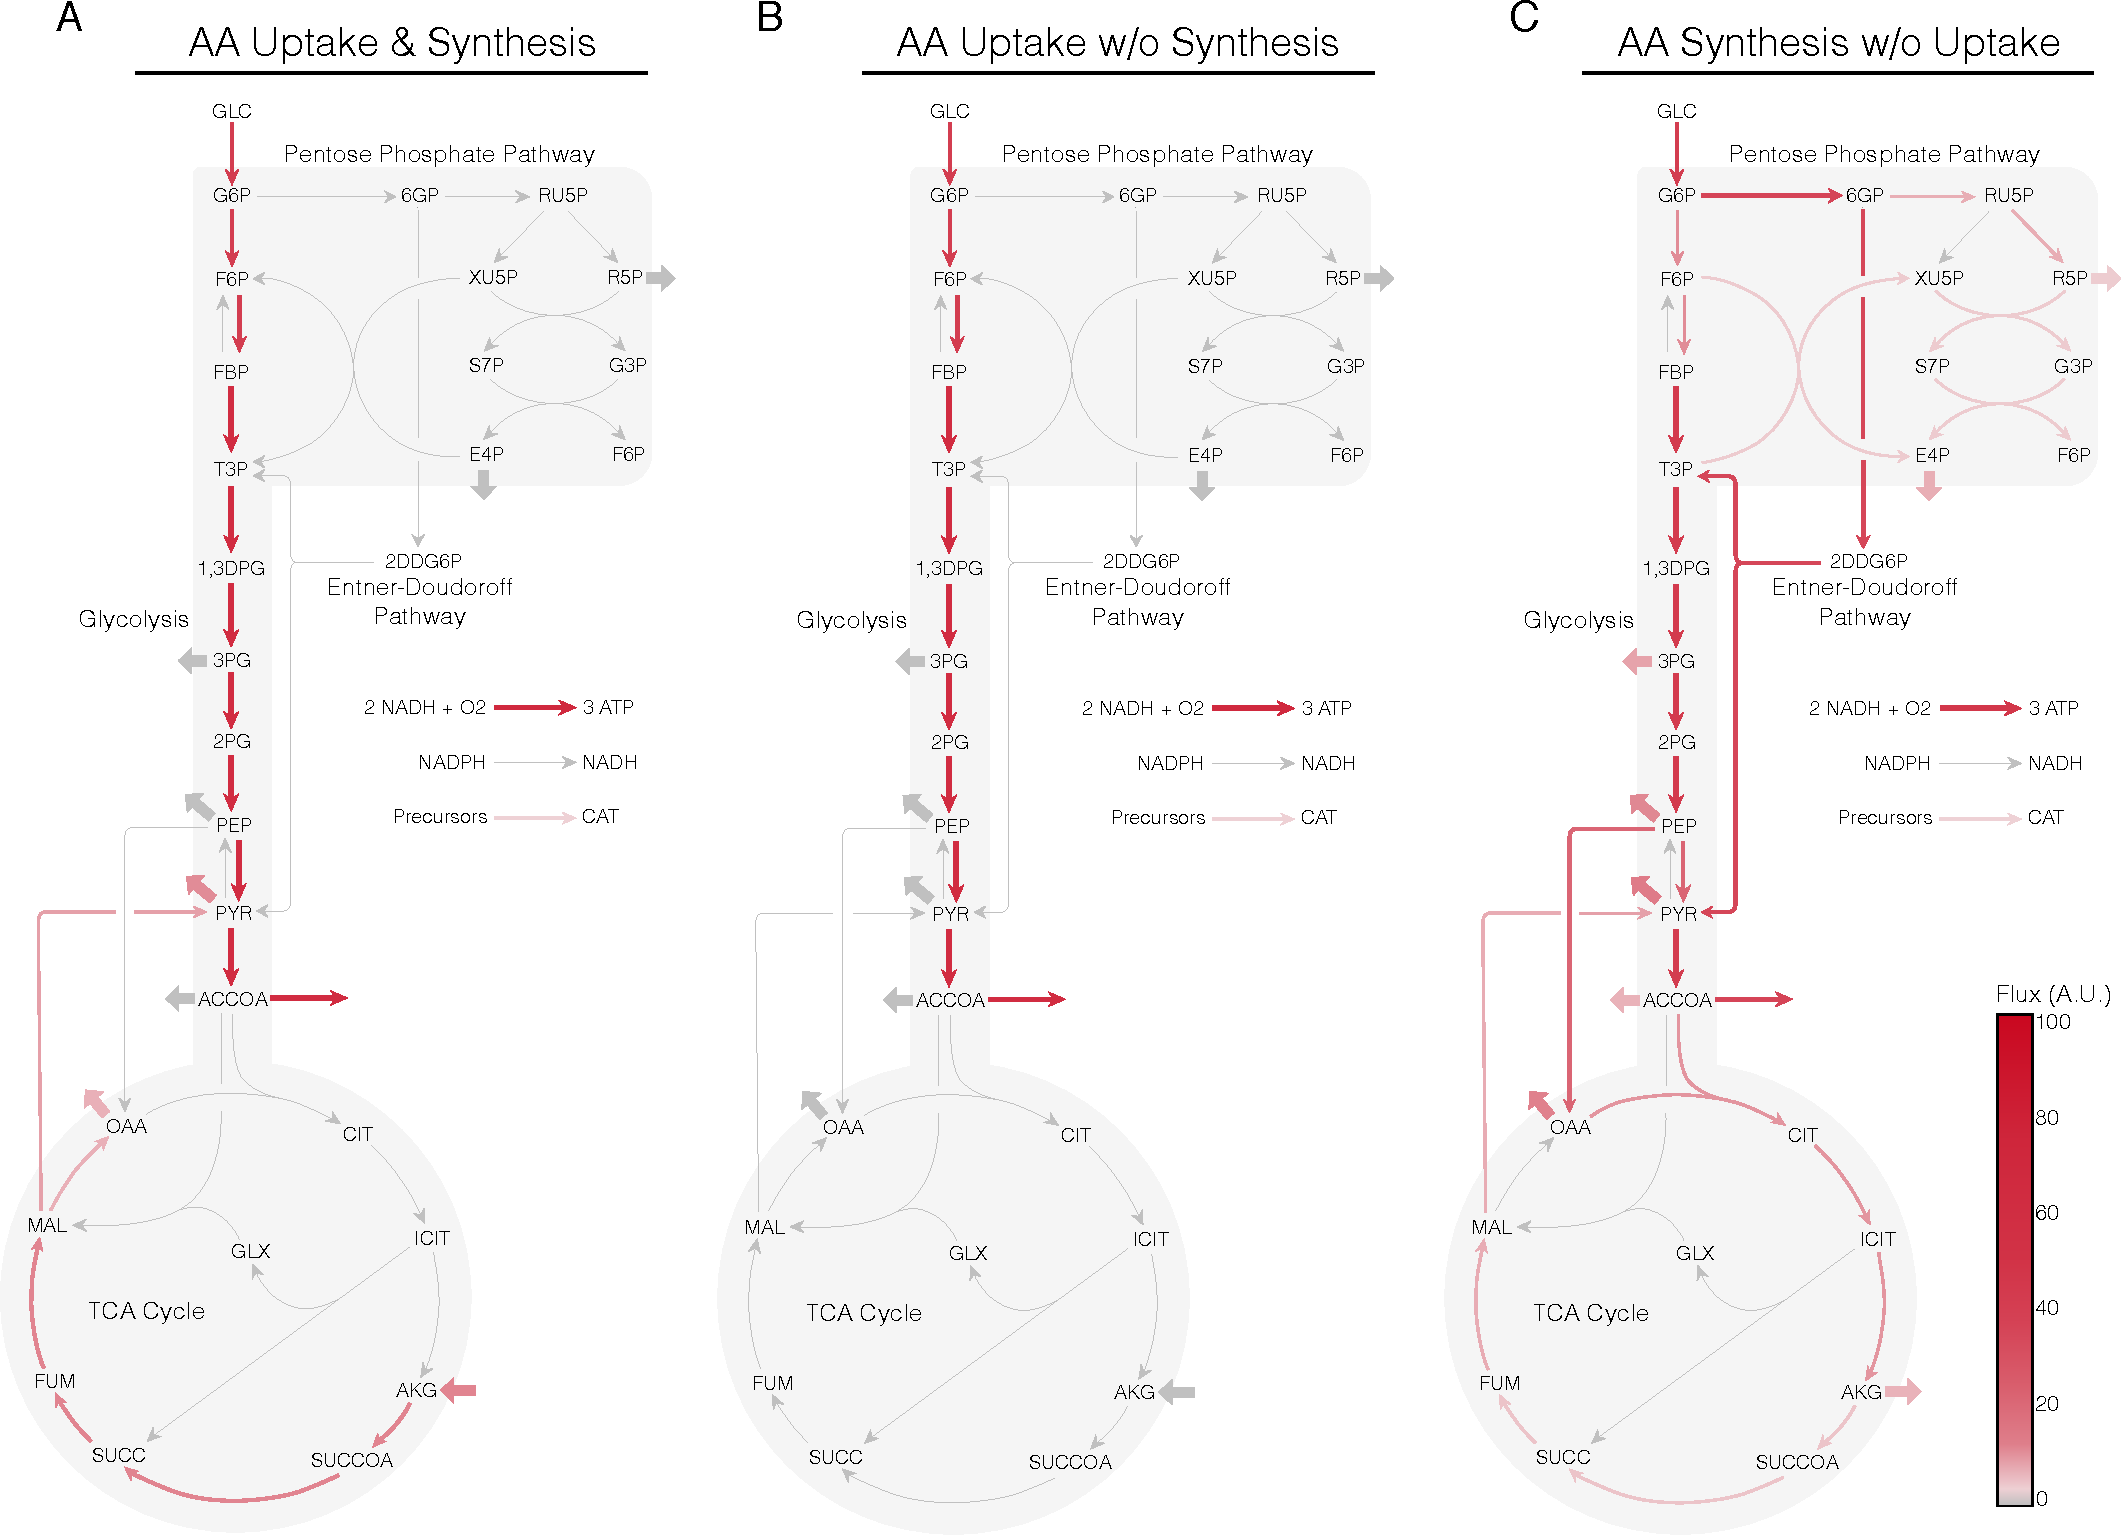
\includegraphics[width=1.00\textwidth]{./Figures/Flux.pdf}
\caption{Flux profile for glycolysis, pentose phosphate pathway, Entner-Doudoroff pathway, TCA cycle, and oxidative phosphorylation, for three different cases: (A) amino acid uptake and synthesis, (B) amino acid uptake without synthesis, and (C) amino acid synthesis without uptake. Mean flux across the ensemble, normalized to glucose uptake flux. Thick arrows indicate flux to or from amino acids.}
\label{fig:flux}
\end{figure}
The first case, which was supplied with amino acids and could synthesize them in the network, relied on a combination of glucose and amino acids to power the system (Fig.~\ref{fig:flux}A).
Glucose traveled through glycolysis and the Entner-Doudoroff pathway to generate NADH for oxidative phosphorylation as well as utilize pyruvate for amino acid biosynthesis.
Interestingly, amino acids rather than glucose powered the TCA cycle, via alpha-ketoglutarate and fumarate, and by utilizing oxaloacetic acid for additional amino acid biosynthesis.
Thus, ssFBA found that the combined utilization of glucose and amino acids to energize CFPS was the optimal case for protein synthesis.
In the second case, where amino acid synthesis was removed from the network, glucose was solely utilized to provide the necessary energy requirements via glycolysis which generated enough NADH for oxidative phosphorylation.
Ubiquinone was generated via \textit{nuo} to power oxidative phosphorylation, instead of relying on the TCA cycle.
Once the energy requirements for transcription and translation were met, amino acids were taken from the media to assemble the protein of interest.
The first two cases had similar performance in terms of productivity, energy efficiency and carbon yield for all proteins.
This is most likely due to the efficient utilization of carbon to energize CFPS without the burden of amino acid biosynthesis.
In the third case, where amino acids must be synthesized, there is drop in all performance metrics (productivity, energy efficiency, and carbon yield) compared to the first two cases.
%Glucose passes through all the major pathways: glycolysis, pentose phosphate pathway and the TCA cycle.
%First, glucose must be converted into all the necessary amino acids for the assembly of the protein of interest.
%Second, it must provide the necessary energy requirements for transcription and translation.
This drop in performance is due to the burden of synthesizing amino acids, which require NADPH.
This leads to the relatively high flux for the conversion of NADH to NADPH.
Thus, less NADH is available for oxidative phosphorylation.
%, thus requiring glucose to energize CFPS as well as synthesize amino acids results in a decrease in performance.
The performance metrics and sensitivity analysis suggest that efficient energy generation via oxygen uptake is essential to higher energy efficiency and carbon yields.
Thus, removing anaerobic enzymes during the cell-free extract preparation could potentially improve CFPS performance and protein yield.

The fourth case, constrained by experimental measurements (Fig. \ref{fig:flux_exp}), had a fairly similar flux distribution as the third case.
The central carbon organic acids show good agreement with the data (Fig. \ref{fig:flux_exp}B).
Metabolic fluxes were constrained by experimental measurements (available in Supporting Information) where available for the first hour which constrained the solution space of ssFBA to have a more realistic depiction of the flux distribution.
Unlike the second case, only certain amino acid synthesis reactions were blocked since during the growth of \emph{E.~coli} not all amino acids were supplied.
During the cell-free reaction all amino acids were supplied, however glucose still traveled through all the major pathways, and the same metabolic precursors were still utilized for amino acid biosynthesis.
Accumulation of pyruvate, lactate, acetate, and other organic acids can be seen (Fig. \ref{fig:flux_exp}B), implying an inefficiency of carbon utilization.
In addition, there is a high flux through the Entner-Douodoroff pathway, but this is likely non-physiological, and simply an artifact of the optimal solution of ssFBA.
To determine which reactions occur in CFPS, adding thermodynamic feasibility constraints to reactions may result in a better depiction of the intracellular flux distribution \cite{Henry:2007,Hamilton:2013}.
In this case, it is unclear which substrate (glucose or amino acids) is used to power CFPS and may in fact be a combination of both.
Thus, it would be interesting to track the carbon flux using C\textsuperscript{13} labeling in CFPS and constrain branch reactions in ssFBA to the resulting measurements, a method that has been shown to represent the flux distribution for \emph{in~vivo} processes well \cite{Zamboni:2009}.
\begin{figure}[t!]
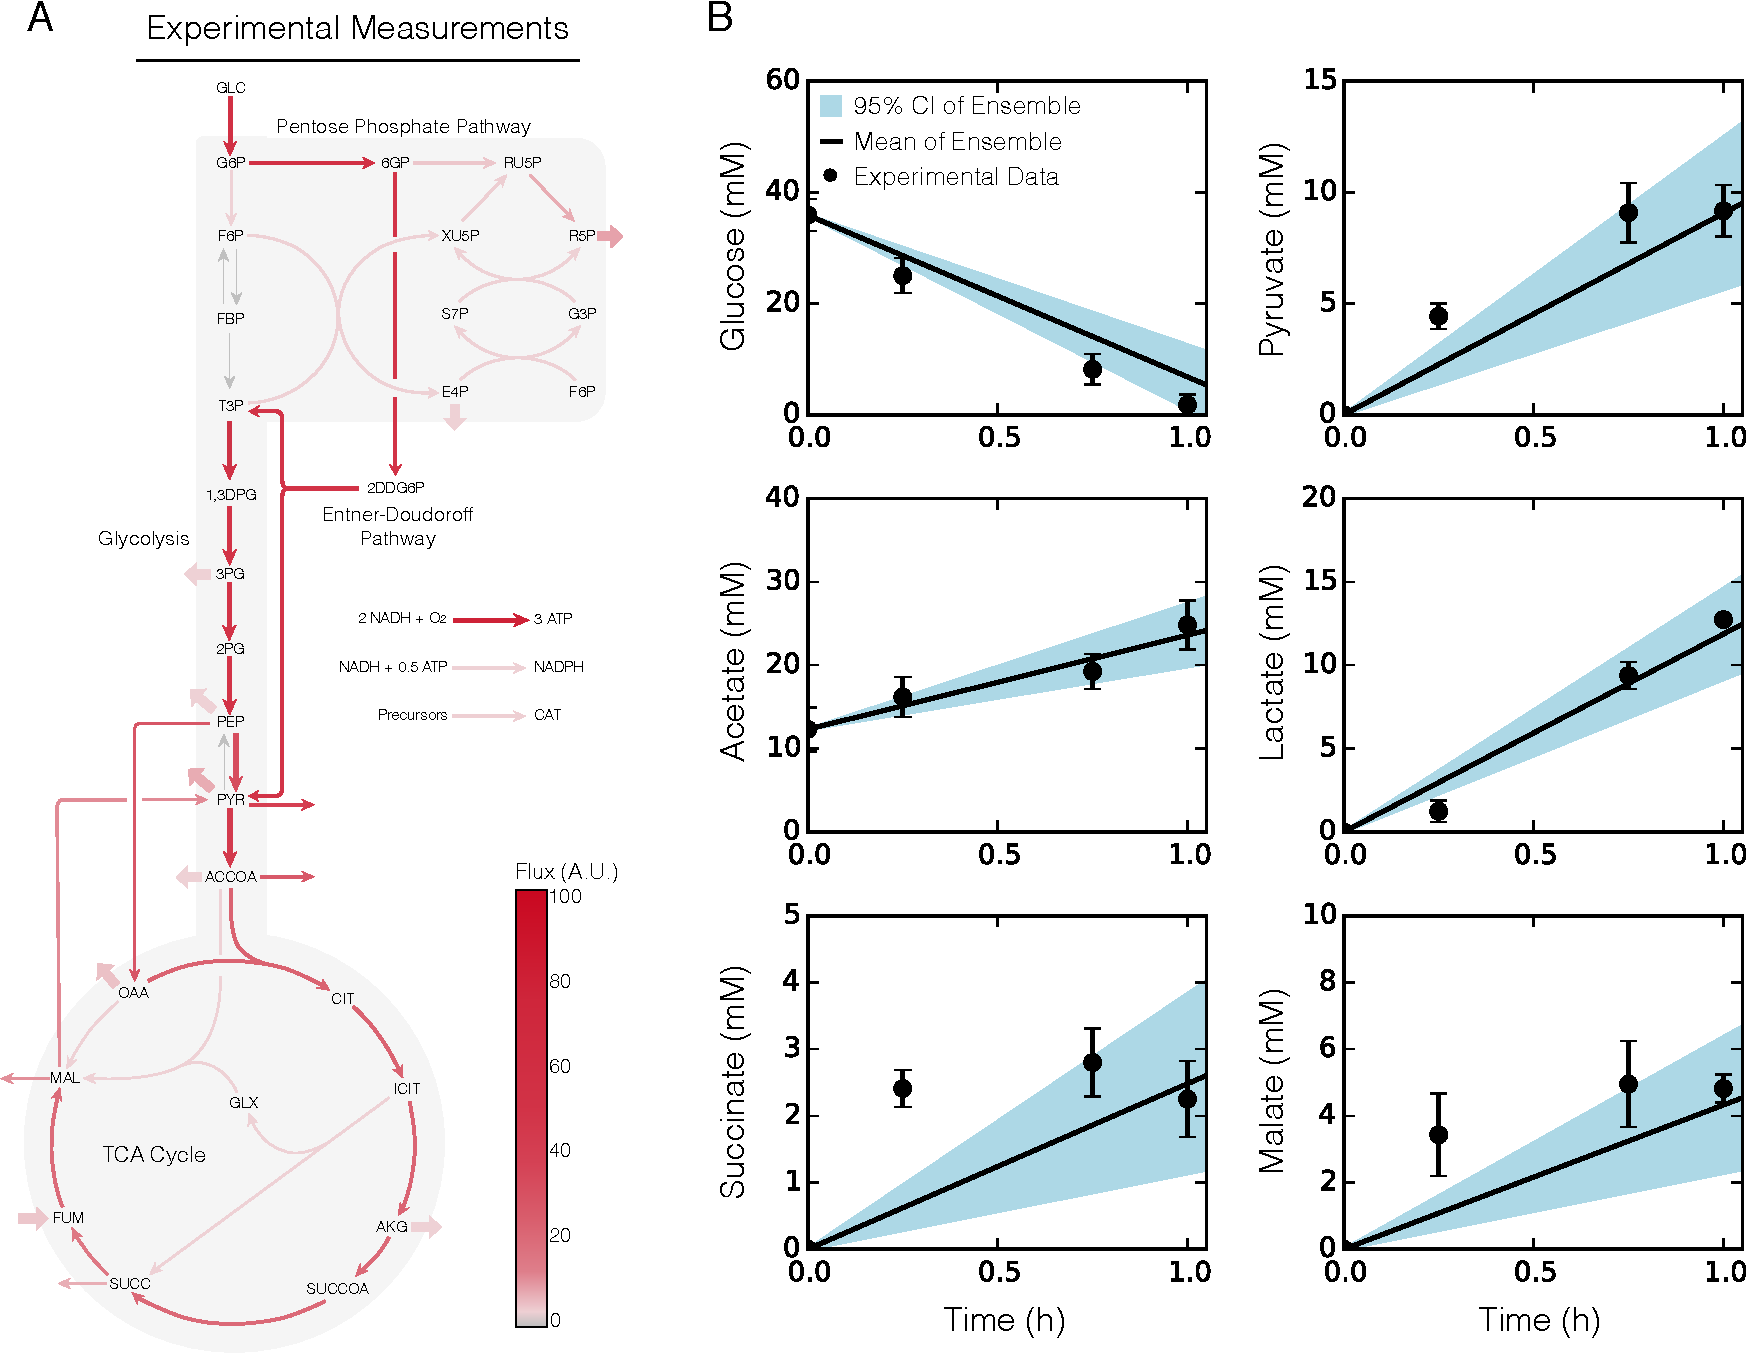
\includegraphics[width=1.00\textwidth]{./Figures/ssFBA_exp.pdf}
\caption{ssFBA simulation of CAT production for an experimentally constrained case. (A) Flux profile for glycolysis, pentose phosphate pathway, Entner-Doudoroff pathway, TCA cycle, and oxidative phosphorylation.  Mean flux across the ensemble, normalized to glucose uptake flux. Thick arrows indicate flux to or from amino acids. (B) Central carbon metabolite measurements versus ssFBA simulations over a one hour time course.}
\label{fig:flux_exp}
\end{figure}

Taken together, we developed a sequence specific constraints based modeling approach to evaluate the performance of synthetic circuits in an \emph{E.~coli} CFPS system for a range of different proteins and three different cases.
We have shown first principle predictions for protein production of deGFP and CAT in agreement with experimental measurements, under two different promoters and two different cell-free extract systems, with few adjustable parameters in the promoter models taken from literature.
This modeling approach suggested trends for productivity, energy efficiency and carbon yield as a function of carbon number.
Furthermore, global sensitivity analysis identified oxygen uptake as being instrumental for maintaining a high energy efficiency and carbon yield.
The translation rate was identified as the rate limiting step for productivity.
The model also suggested that cell-free systems can simultaneously operate aerobically and anaerobically, which can lead to inefficient production and should be addressed to optimize energy efficiency and carbon yield.
In conclusion, sequence specific constraints based modeling offers a novel means to \emph{a~priori} estimate the performance of cell-free synthetic circuits.

\section*{Materials and Methods}

\subsection*{Formulation and solution of the model equations.}
We estimated the theoretical maximum performance of the cell-free protein synthesis system using sequence specific flux balance analysis (ssFBA) \cite{Allen:2003aa}.
The sequence specific flux balance analysis problem was formulated as a linear program:
\begin{equation}
 \begin{multlined}
	\qquad \qquad \qquad \max_{\boldsymbol{w}}{} \! \left( w_{TL} = \mathbf{\boldsymbol{\theta}}^T \boldsymbol{w} \right) \\
	\mathrm{Subject \; to:}
	 \; \; \mathbf{S}\mathbf{w}=\mathbf{0} \\
\alpha_i \leq w_i \leq \beta_i  \qquad i=1,2,\hdots,\mathcal{R}
 \end{multlined}
\end{equation}
where $\mathbf{S}$ denotes the stoichiometric matrix, $\mathbf{w}$ denotes the unknown flux vector, $\boldsymbol{\theta}$ denotes the objective selection vector
and $\alpha_i$ and $\beta_i$ denote the lower and upper bounds on flux $w_{i}$, respectively.
The stoichiometry of the kinetic model was used for the ssFBA calculations, with the execpetion of the transcription and translation rates.
The transcription (TX) and translation (TL) stoichiometry was modeled using the template reactions taken from Allen and Palsson \cite{Allen:2003aa}:
\begin{eqnarray*}
\mathrm{{G}_{\mathcal{P}}}+\mathrm{{R}_{1}} &\longrightarrow& \mathrm{G_{\mathcal{P}}^{*}} \\
\mathrm{G_{\mathcal{P}}^{*}}+\sum_{\mathrm{k\in\left\{A,C,G,U\right\}}}\eta_{k}\cdot \mathrm{\left\{k\right\}TP} &\overset{\rm TX}{\longrightarrow}& \mathrm{mRNA}+\mathrm{G_{\mathcal{P}}}+\mathrm{R_{1}}+ \mathrm{\sum_{k\in\left\{A,C,G,U\right\}}2\eta_{k}\cdot Pi}\\
\mathrm{mRNA} &\longrightarrow& \mathrm{\sum_{k\in\left\{A,C,G,U\right\}}\eta_{k}\cdot \left\{k\right\}MP} \\
\mathrm{mRNA}+\mathrm{R_{2}} &\longrightarrow& \mathrm{R_{2}^{*}} \\
\mathrm{\alpha_{j}\cdot AA_{j}+\alpha_{j}\cdot tRNA+\alpha_{j}\cdot ATP} &\longrightarrow& \mathrm{\alpha_{j}\cdot AA_{j}-tRNA_{j}+}\\
&& \mathrm{\qquad \alpha_{j}\cdot AMP+2\alpha_{j}\cdot Pi} \qquad{j=1,2,\hdots,20}\\
\mathrm{R_{2}^{*}+\sum_{j\in\left\{AA\right\}}\alpha_{j}\cdot \Big(AA_{j}-tRNA_{j}+2\cdot GTP\Big)} &\stackrel{\rm TL}{\longrightarrow}& \mathcal{P}+\mathrm{R_{2}+mRNA}+\\
&& \mathrm{\quad +\sum_{j\in\left\{AA\right\}}\alpha_{j}\cdot\Big(tRNA+2\cdot GDP+2\cdot Pi\Big)}
\end{eqnarray*}
where $G_{\mathcal{P}}$ denotes the gene encoding protein product $\mathcal{P}$,
$\rm R_{1}$ denotes the concentration of RNA polymerase,
$G_{\mathcal{P}}^{*}$ denotes the gene bounded by the RNA polymerase,
$\eta_{i}$ and $ \alpha_{j}$ denote the stoichiometric coefficients for nucleotide and amino acid, respectively,
$\rm Pi$ denotes inorganic phosphate,
$\rm R_{2}$ denotes the ribosome concentration,
$\rm R_{2}^{*}$ denotes bounded ribosome,
and $AA_{j}$ denotes the $j^{th}$ amino acid.

The transcription rate ($w_{TX}$) was fixed in the ssFBA calculation at:
\begin{equation}
	w_{TX} = V_{TX}^{max}\left(\frac{G}{K_{TX}+G}\right)
\end{equation}
where $G$ denotes the gene concentration and $K_{TX}$ denotes a transcription saturation coefficient.
The maximum rate of transcription $V_{TX}^{max}$ was formulated as:
\begin{equation}
	V_{TX}^{max} \equiv \left[R_{1}\left(\frac{v_{TX}}{l_{G}}\right)\mathcal{P}\right]
\end{equation}
The term $R_{1}$ denotes the RNA polymerase abundance,
$v_{TX}$ denotes the RNA polymerase elongation rate (nt/h),
$l_{G}$ denotes the gene length in nucleotides, and the last term $\mathcal{P}$ describes a model of promoter activity.
In this study, we considered two promoters: T7 and $\sigma_{70}$.
The promoter function for the T7 promoter, $\mathcal{P}_{T7}$, was given by:
\begin{equation}
	P_{T7} = \frac{K_{T7}}{1 + K_{T7}}
\end{equation}
where $K_{T7}$ denotes a T7 RNA polymerase binding constant \cite{Moon:2012aa}.
The $\sigma_{70}$ binding promoter, used for all other proteins, was formulated as:
\begin{equation}
	P_{\sigma_{70}} = \frac{K_{1}+K_{2}f_{p70}}{1 + K_{1}+K_{2}f_{p70}}
\end{equation}
where $K_{1}$ denotes the state of RNA polymerase binding,
$K_{2}$ is the state of $\sigma_{70}$ binding along with RNA polymerase, and $f_{p70}$ denotes the fraction of the $\sigma_{70}$ transcription factor bound to the promoter (modeled as a Hill function).

The translation rate ($w_{TL}$) was bounded by:
 \begin{equation}
	0\leq w_{TL} \leq V_{TL}^{max}\left(\frac{\rm mRNA_{SS}}{K_{TL}+\rm mRNA_{SS}}\right)
\end{equation}
where $\rm mRNA_{SS}$ denotes the steady state mRNA abundance and $K_{TL}$ denotes the translation saturation constant.
The maximum translation rate $V_{TL}^{max}$ was formulated as:
\begin{equation}
	V_{TL}^{max} \equiv \left[K_{P} R_{2}\left(\frac{v_{TL}}{l_{P}}\right)\right]
\end{equation}
The term $K_{P}$ denotes the polysome amplification constant,
$v_{TL}$ denotes the ribosome elongation rate (amino acids per hour),
$l_{P}$ denotes the number of amino acids in the protein of interest,
and $\rm mRNA_{SS}$ denotes the steady-state mRNA concentration:
\begin{equation}
	 mRNA_{SS}\simeq\frac{w_{TX}}{\lambda}
\end{equation}
where $\lambda$ denotes the rate constant controlling the mRNA degradation rate.

The objective of the sequence specific flux balance calculation was to maximize the rate of protein translation, $w_{TL}$.
The total glucose uptake rate was bounded by [0,40 mM/h] according to experimental data, while the amino acid uptake rates were bounded by [0,30 mM/h], but did not reach the maximum flux.
Gene and protein sequences were taken from literature and are available in the Supporting Information.
The sequence specific flux balance linear program was solved using the GNU Linear Programming Kit (GLPK) v4.55 \cite{GLPK}.
For all cases, amino acid degradation reactions were blocked since these enzymes were knocked out during the cell-free extract preparation \cite{2005_calhoun_BiotechnologyProgress, Garamella:2016aa}.
In the second case, all amino acid synthesis reactions were set to 0 mM/hr since \textit{E. coli} was grown in the presence of amino acids, thus these enzymes would not be present in the cell-free extract media.
In the third case, amino acid uptake reactions were set to 0 mM/hr.   
In the experimental constrained case, \textit{E. coli} was grown in the presence of 13 amino acids (alanine, arginine, cysteine, serine, aspartate, glutamate, and glutamine were excluded) \cite{Zawada:2003}, thus the synthesis reactions responsible for those 13 amino acid were set to 0 mM/hr.  

\subsection*{Calculation of energy efficiency.}
Energy efficiency was calculated as the ratio of protein production to glucose consumption, both in terms of equivalent ATP molecules:
\begin{equation}\label{eqn:energy-efficiency-definition}
	Efficiency=\frac{\Delta\texttt{POI}\cdot \left(2\left({ATP}_{TX}+\rm {CTP}_{TX}+\rm {GTP}_{TX}+\rm {UTP}_{TX}\right)+\rm2\cdot\rm {ATP}_{TL}+\rm {GTP}_{TL}\right)}{\Delta\texttt{GLC}\cdot\texttt{ATP}_{GLC}}
\end{equation}
where $\Delta\texttt{POI}$ denotes the flux of the protein of interest produced, $\rm {ATP}_{TX}$, $\rm {CTP}_{TX}$, $\rm {GTP}_{TX}$, $\rm {UTP}_{TX}$ denote the stoichiometric coefficients of each energy species for the transcription of the protein of interest, $\rm {ATP}_{TL}$, $\rm {GTP}_{TL}$ denote the stoichiometric coefficients of ATP and GTP for the translation of the protein of interest, $\Delta\texttt{GLC}$ denotes the glucose flux, and $\rm {ATP}_{GLC}$ denotes the equivalent ATP number for glucose.
The energy species stoichiometric coefficients are available in the Supporting Information.

\subsection*{Calculation of the carbon yield.}
The carbon yield ($Y_{C}^{POI}$) was calculated as the ratio of carbon produced as the protein of interest divided by the carbon consumed as reactants (glucose and amino acids):
\begin{equation}\label{eqn:yield-definition}
	Y_{C}^{POI}=\frac{\Delta\texttt{POI}\cdot C_{POI}}{\displaystyle\sum_{i=1}^{\mathcal{R}}\max(\Delta m_{i},0)\cdot C_{m_i}}
\end{equation}
where $\Delta\texttt{POI}$ denotes the flux of the protein of interest produced, $C_{POI}$ denotes carbon number of the protein of interest, $\mathcal{R}$ denotes the number of reactants,
$\Delta m_{i}$ denotes the amount of the $i^{th}$ reactant consumed (not allowed to be negative), and $C_{m_i}$ denotes the carbon number of the $i^{th}$ reactant.


\subsection*{Quantification of uncertainty.}
An ensemble of 100 sets of flux distributions was calculated for each of the three different cases: control (with amino acid synthesis and uptake), amino acid uptake without synthesis, and amino acid synthesis without uptake.
The ensemble was calculated by randomly sampling the maximum specific glucose uptake rate from within a range of 0 to 30 mM/h, determined from experimental data and randomly sampling RNA polymerase levels, ribosome levels, and elongation rates in a physiological range determined from literature.
RNA polymerase levels were sampled between 60 and 80 nM, ribosome levels between 7 and 16 \textmu M, the RNA polymerase elongation rate between 20 and 30 nt/sec, and the ribosome elongation rate between 1.5 and 3 aa/sec \cite{2005_underwood_biotech, Garamella:2016aa}.

\subsection*{Global sensitivity analysis.}
We conducted a global sensitivity analysis using the variance-based method of Sobol to estimate which parameters controlled the performance of synthetic circuits \citep{SOBOL_METHOD}.
We computed the total sensitivity index of each parameter relative to three performance objectives: productivity of the protein of interest, energy efficiency and carbon yield.
We established the sampling bounds for each parameter from literature.
We used the sampling method of Saltelli \textit{et al.} \citep{Saltelli:2010} to compute a family of $N\left(2d+2\right)$ parameter sets which obeyed our parameter ranges,
where $N$ was a parameter proportional to the desired number of model evaluations and $d$ was the number of parameters in the model. In our case, $N$ = 1000 and $d$ = 7, so the total sensitivity indices were computed from 16,000 model evaluations. The variance-based sensitivity analysis was conducted using the SALib module encoded in the Python programming language \citep{SALIB}.

%%%%%%%%%%%%%%%%%%%%%%%%%%%%%%%%%%%%%%%%%%%%%%%%%%%%%%%%%%%%%%%%%%%%%
%% The "Acknowledgement" section can be given in all manuscript
%% classes.  This should be given within the "acknowledgement"
%% environment, which will make the correct section or running title.
%%%%%%%%%%%%%%%%%%%%%%%%%%%%%%%%%%%%%%%%%%%%%%%%%%%%%%%%%%%%%%%%%%%%%
\begin{acknowledgement}

Please use ``The authors thank \ldots'' rather than ``The
authors would like to thank \ldots''.

The author thanks Mats Dahlgren for version one of \textsf{achemso},
and Donald Arseneau for the code taken from \textsf{cite} to move
citations after punctuation. Many users have provided feedback on the
class, which is reflected in all of the different demonstrations
shown in this document.

\end{acknowledgement}

%%%%%%%%%%%%%%%%%%%%%%%%%%%%%%%%%%%%%%%%%%%%%%%%%%%%%%%%%%%%%%%%%%%%%
%% The same is true for Supporting Information, which should use the
%% suppinfo environment.
%%%%%%%%%%%%%%%%%%%%%%%%%%%%%%%%%%%%%%%%%%%%%%%%%%%%%%%%%%%%%%%%%%%%%
\begin{suppinfo}
The following files are available free of charge.
\begin{itemize}
  \item Protein Sequences: DNA and protein sequences of each protein of interest.
  \item Supporting Information: Performance trendlines as a function of carbon number and transcription/translation stoichiometric coefficients of energy species.
  \item Carbon Yield Sensitivity Analysis: Global sensitivity analysis on deGFP carbon yield.
\end{itemize}
\end{suppinfo}

%%%%%%%%%%%%%%%%%%%%%%%%%%%%%%%%%%%%%%%%%%%%%%%%%%%%%%%%%%%%%%%%%%%%%
%% The appropriate \bibliography command should be placed here.
%% Notice that the class file automatically sets \bibliographystyle
%% and also names the section correctly.
%%%%%%%%%%%%%%%%%%%%%%%%%%%%%%%%%%%%%%%%%%%%%%%%%%%%%%%%%%%%%%%%%%%%%
\bibliography{References_v1}

\end{document}
\grid
